The chapter will present the \acrlong{vr} system architecture, then I will talk about the hardware and software used during the development and prototyping process. I will show in detail the development process of Glimpses from Palestine application, from developing the \acrshort{vr} environment to re-building Al-Ghabisiyya in \acrlong{vr}. In the last section, I will talk about the design of the application \acrlong{ui}.

\section{Virtual Reality components}



Two main subsystems, hardware and software, make up a \acrshort{vr} system. The hardware can also be divided into \acrshort{vr} engine and I/O devices, while the software can be split into application software and database as shown in Figure \ref{fig:sys}. A \acrshort{vr} system's classic five components are Software and Database, VR Engine, I/O Devices, User and Task \citep{burdea2017virtual,Bamodu2013VirtualComponents}.

\begin{figure}[ht]
    \centering
    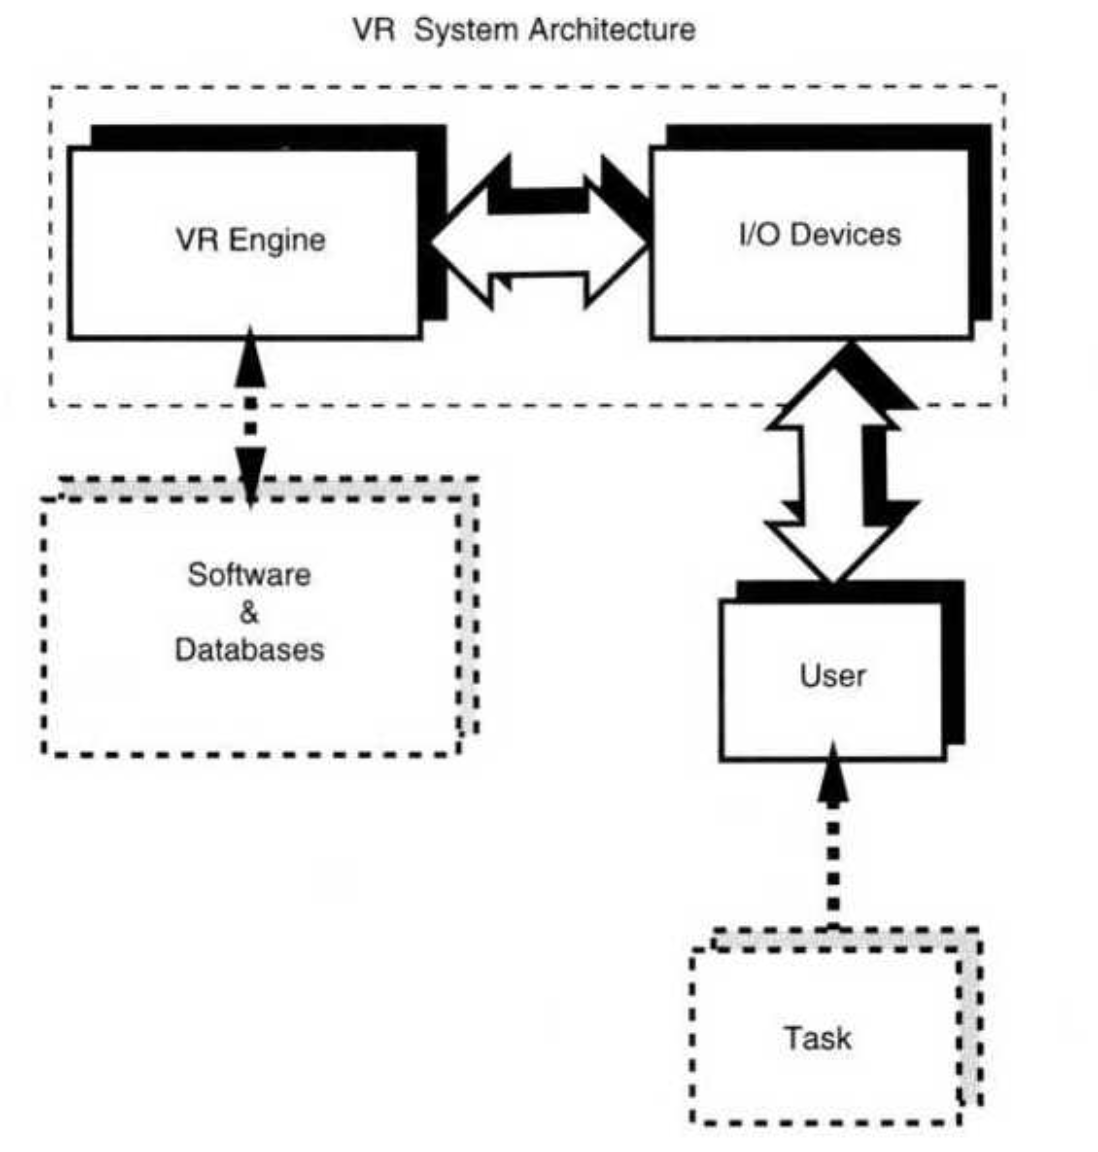
\includegraphics[width=0.50\textwidth]{images/VR.png}
    \caption{VR System Architecture - \citep{burdea2017virtual}}
    \label{fig:sys}
\end{figure}


\subsection{Software and Database}
Application for Virtual Reality Project is a set of tools and software to plan, develop and maintain virtual environments and the database where the information is stored. The tools can be classified as tools for modeling and development. There are many modeling tools available for \acrshort{vr} development, with 3D Max, Maya, and Creator being the most popular. Solidworks, Fusion 360, and CATIA are Engineering specific applications that could be used as well. \acrshort{vr} is a dynamic and integrative technology that borrows from many other innovations, such as real-time 3D computer graphics, tracking technology, motion synthesis, and haptic engineering, among others \citep{burdea2017virtual, Bamodu2013VirtualComponents}.

\subsection{VR Engine}
 The \acrshort{vr} engine or computer system must be selected in \acrshort{vr} systems according to the application's requirement. Some of the most important factors and time-consuming activity in a \acrshort{vr} environment is graphic interface and image creation. The selection of the \acrshort{vr} engine depends on the application area, user I/O devices immersion level, and the appropriate graphical output, as it is responsible for measuring and creating visual models, rendering objects, lighting, visualization, shading, simulation and show in real-time. The computer also manages interaction with users and serves as an interface to I/O devices. The processing power of the computer is a big factor to consider when choosing the \acrshort{vr} engine, and the processing power of the computer is the number of senses (graphic, audio, etc.) that can be rendered as pointed in a specific time frame. The \acrshort{vr} engine is expected to recalculate the virtual world roughly every 33ms and generate more than 24fps of real-time simulation, and the corresponding graphic engine should also be able to produce stereoscopic vision. The \acrshort{vr} engine could be a regular PC with more processing power and an efficient processor for graphics or decentralized computer systems linked through a high-speed communication network \citep{burdea2017virtual, Bamodu2013VirtualComponents}.


\subsection{I/O Devices}
 The input tools are the way for communicating with the virtual world by the user. They send signals about the user's action to the system to provide the user with appropriate reactions in real-time via the output devices. They can be categorized into devices for tracking, point-input devices, bio-controllers and voice devices. Often referred to as location sensors, tracking devices are used to detect the user's position, including electromagnetic, ultrasonic, optical, mechanical and gyroscopic detectors, data goggles, neural and bio or muscle controls. Types of point-input devices provide 6 \acrfull{dof} and space or force ball. Their technology is a normal mouse adaptation with extended functionality and 3D capability. Communication of voice is a common way of human interaction. Therefore, incorporating it into a \acrshort{vr} device also feels natural. To accomplish this, voice recognition or processing software may be used \citep{burdea2017virtual, Bamodu2013VirtualComponents} .

 The output devices receive feedback from the \acrshort{vr} engine and pass it on to users to stimulate the senses through the appropriate output devices. The possible senses-based classifications of output devices are graphics (visual), audio (aural), haptic (contact or force), odor and taste. The first 3 of these are often used in \acrshort{vr} environments, though odor and taste are still rare.The stereo video screen and the \acrfull{hmd}, which offers a higher level of immersion, are two potential traditional graphics choices. In the \acrshort{hmd}, the brain interprets the two separate views generated to provide a 3D perspective of the virtual world. An important medium in \acrshort{vr} is audio or sound, its value is only matched by that of video. To make the VR experience more immersive, 3D audio can be used to produce different sounds from different locations \citep{burdea2017virtual, Bamodu2013VirtualComponents}.



\subsection{User}

The users are the main reason to keep or to improve a particular \acrshort{vr} system design depending on their responses. Some users might have motion sickness during the simulation, therefore we should know what caused it, and how to avoid it. Human behavior can not be measured mathematically, it is a qualitative data, therefore its more difficult to analyze the human-machine interaction. \acrshort{vr} has many parameters, however, \acrshort{vr} human factor studies is a series of experiments aimed at determined users to perform with \acrshort{vr} technology, and it tests usability, user safety, and any related social impact related to \acrshort{vr}. 

\begin{figure}[ht]
    \centering
    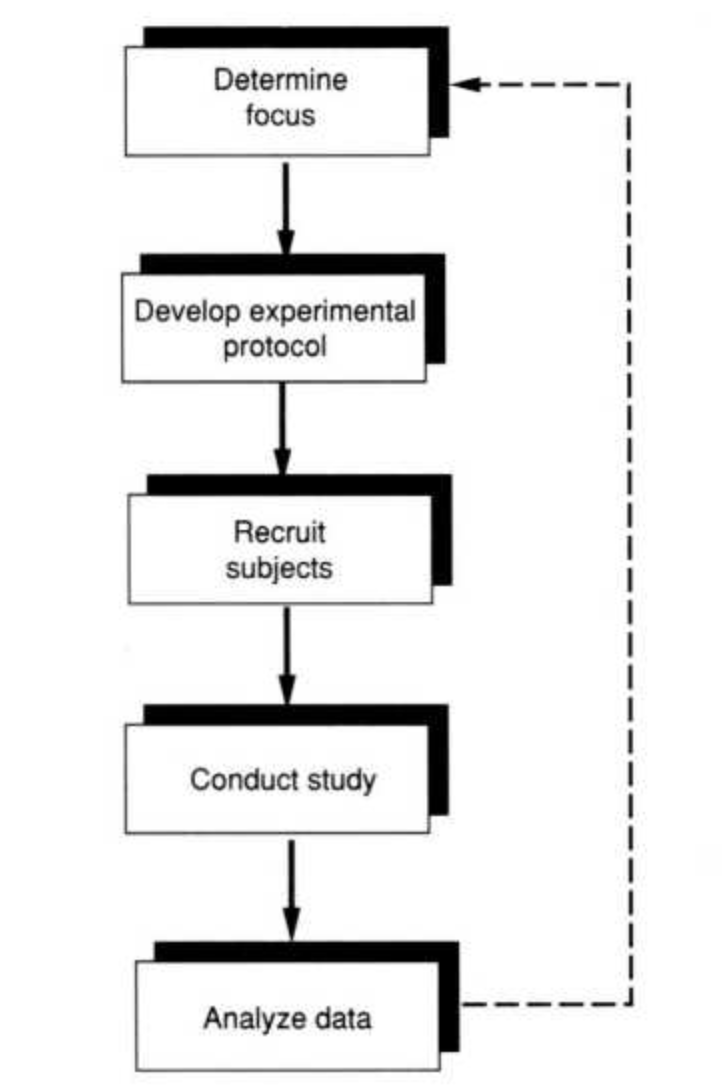
\includegraphics[width=0.40\textwidth, height=250pt]{images/VRhf.png}
    \caption{VR human factors study - \citep{burdea2017virtual}}
    \label{fig:vrhf}
\end{figure}

A great advantage of data collection in \acrlong{vr} that it can be sampled during the testing, also the researcher can have a comprehensive view while the user is immersed in the simulation. Nevertheless, while designing the experimental protocol the researcher should avoid any drawbacks, for instance, to not have a repeated subject, because it will end up with the same results because data validity comes with the subject actions. Also to avoid hardware and software problems like latency which will affect the validity and reliability of the experiment. After the data is collected and analyzed, the findings will be used to refine the user interface design, enhance the software performance or add any new features to the application \citep{burdea2017virtual}. 
 
\subsection{Task}

I talked about different applications and platforms that \acrshort{vr} made an impact on it in Chapter \ref{StateoftheArt}. There are more tasks that \acrlong{vr} can enhance their performance.

For instance, Virtual reality in manufacturing. The life cycle of the manufacturing system is based on different stages, like design, personnel training, and operation, but there are multiple domains of \acrshort{vr} in manufacturing as shows in Figure \ref{fig:vrman}. 
\begin{figure}[ht]
    \centering
    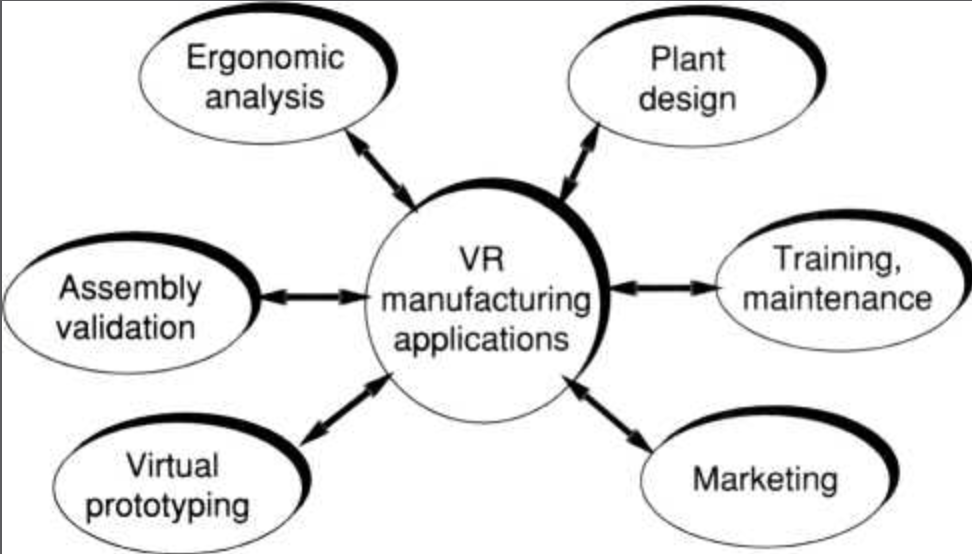
\includegraphics[width=0.50\textwidth]{images/VRmanu.png}
    \caption{Domains of VR in manufacturing - \citep{burdea2017virtual}}
    \label{fig:vrman}
\end{figure}

\textbf{Virtual prototyping}: It is an obligatory stage of the development process, where the designer can validate the design, and establish manufacturing methods. Instead of drawing on a paper Virtual reality allow the designers to receive a simulation and quick feedback for the design.


\textbf{Assembly validation}: Another stage of prototyping, if the product contains multiple parts, in this stage the separate designed parts need to be tested and see they all fit together. \acrshort{vr} allows the user to test and assemble the parts. If there are flaws found in the design, it can be modified directly. 


\textbf{Ergonomic analysis}: This is made after the physical prototype is done and exist. Virtual Reality gives the users control and feels the ergonomics of the prototype in real-time. The ergonomic analysis depends on body discomfort during the testing time. With different tools, the body ergonomics of the user and the comfort of the body is being tested during the simulation in \acrshort{vr}. 

\textbf{Plant design}: New factories and large industries need to have a plan for the construction and the flow of tasks inside the facility. That's where Virtual reality can be used for simulating the tasks flow, and the user can control equipment. Designers can run high complexity tasks that cover safety, production, and many dynamic variables. Everything can be simulated by \acrshort{vr}, before anything goes into production.  

\textbf{Training maintenance}:  Training of employees takes a lot of time and effort, also it might be dangerous. Using Virtual reality in training for the assembly line, reducing the number of errors, and the training was more efficient compared to the standard training.

\textbf{Marketing}: Virtual reality also played a good role in marketing, an example for that was at many car dealerships where they had a virtual reality room, that makes the customer interact with the car within the virtual environments and adjust the car color or the seat material.

\section{Hardware and Development Environments}

In this section, I will mention and define the equipment and tools that I used to develop the application. The software that i used to build the application. and The camera's that was used to film the cities and locations in Palestine. I used Virtual reality headsets and headphones to test the application with users.


\subsection{Headsets}

\textbf{Google Cardboard}: The virtual reality platform was released in
2014 by Google. The platform is intended as a low-cost system to
encourage interest and development in VR applications. It was
named for its fold-out cardboard viewer. The Google Cardboard
headsets are built out of simple, low-cost components -
cardboard. Google open-sourced the schematics and the
assembly instructions freely on their site, allowing people to
assemble Cardboard themselves from readily available parts \citep{Prasuethsut2014GoogleReview}.


\textbf{Google Daydream}: Google Daydream is not made out of plastic and not cardboard. It is made out of cloth, and that makes it a light virtual reality headset. Virtual reality can be activated automatically in android devices with this headset via the \acrfull{nfc} chipset installed on the door of the headset. The smartphone does not need to be in a certain position, because Daydream will automatically align the image of the mobile to the lenses. Since it is made out of cloth, it is a very comfortable headset because of the face cushion that gives a comfortable feeling, and the thick strap that holds the whole headset around the head, like ski goggles. Nevertheless the weight, it makes the user keep playing without being tired \citep{Amadeo2016DaydreamTechnica}. 


\subsection{Cameras}
\textbf{GoPro Fusion}: The footage quality can reach up to 5.2K spherical video resolution. The GoPro fusion can be controlled via a mobile application through Bluetooth or Wi-Fi. The two lenses on the two
sides are not symmetrically aligned, they are off-axis. That helps to
process the images or the footage taken from the two lenses to not
have visible stitching or overlapping in the final image. That is a
common problem in most of the VR cameras to have a big overlapping on the final image. With a 4 microphones built-in the camera, it captures full circle audio for a spatial sound experience. The data is saved on two microSD cards one for each lens, the files need to be combined to have a final 360$^{\circ}$ video \citep{Easton2018}. The camera was used in most of the project filming material, it has the best footage quality and a perfect stabilization in the videos.


\textbf{Samsung Gear 360}: The small and rounded shape of the camera is ideal for handheld shooting, although it has a socket also for a tripod. A small LCD screen helps in navigating through the camera modes. The video resolution is 4K, while the still images are somewhat soft. The smartphone app is easy to use and clear for the user also it offers a good range of viewing options. In general, is it a small and simple camera to use \citep{DigitalCamera2018}. The camera used as a backup camera during the project. The quality is acceptable for a small and very light camera.

\subsection{Development Environments}

\acrshort{vr} technology is moving forward and designers are gradually getting access to new tools and platforms \citep{Bamodu2013VirtualComponents}. Not only in computers but also smartphones and web, \acrshort{vr} technology has found its way into different environments. In this section, I will mention the software's that I used to develop and design a smartphone \acrshort{vr} application \say{Glimpses from Palestine}. 


\textbf{Unity 3D}: Unity is one of the most famous game engines, it is a  fully integrated development engine that offers out-of-the-box capabilities for immersive 3D creations. It has a direct \acrshort{vr} mode to preview the work on any \acrlong{hmd}, which can be easier and faster for designers to boost their productivity \citep{Kim2014UsingDevelopment}. Most of the \acrlong{hmd}s are supported in Unity. Unity works with C\# and JavaScript, it is easy to learn due to the huge online community. Unity can export the work to various platforms including Mac, Web, iOS, Android, and Xbox \citep{Kim2014UsingDevelopment}. Unity's robust tool collection, interactive interface and on-the-fly testing and editing feature let developers save time and effort Unity was the best and most powerful tool to be used during the project to develop the VR experience.

\textbf{Autodesk Fusion 360}: Fusion is a cloud-based 3D modeling software where all your work and files would be saved on the cloud. You can design \acrfull{cad} and \acrfull{cam} for \acrfull{cae} tasks. For my personal experience, it was easier for me to work with Fusion since it is an engineering-based software.  Fusion can animate and make videos, also render high quality images for the designs. Nevertheless, Fusion is designed for all levels of users, from beginner to modeling to experienced engineer \citep{Cline2018FusionFabrication}. 

\section{Development \& Implementation}

 Also, I will present how I did manage to re-build part of the Al-Ghabisiyya village. These tools helped me in modeling the terrain of the geographical area as well as re-building most of the houses of Al-Ghabisiyya. Placing the village on the right location of the map was tricky and challenging therefore, I will explain it in detail. 

\subsection{Glimpses from Palestine Application}

 Having looked closely into the prior design of the \acrshort{vr} application prototype that has been developed during \acrshort{yallah!} I realized that the previous design had many unorganized and missing files. I decided to start the development from scratch again, This will make it more versatile, efficient and quick. Therefore I started to build the 360$^{\circ}$ video environment. In Unity when you start a new scene it has the camera in the middle of the environment by default, this camera will be the user's point of view. The camera will be surrounded by a sphere. The sphere will be the display of the 360$^{\circ}$ video. Since the camera will be in the middle of the sphere and the video will be played on the sphere from outside, the camera will show nothing when you play the scene. Therefore a small C\# code made it possible to flip the player of the video inside the sphere. Then the user will have the feeling of immersion in virtual reality. 
\begin{figure}[ht]
    \centering
    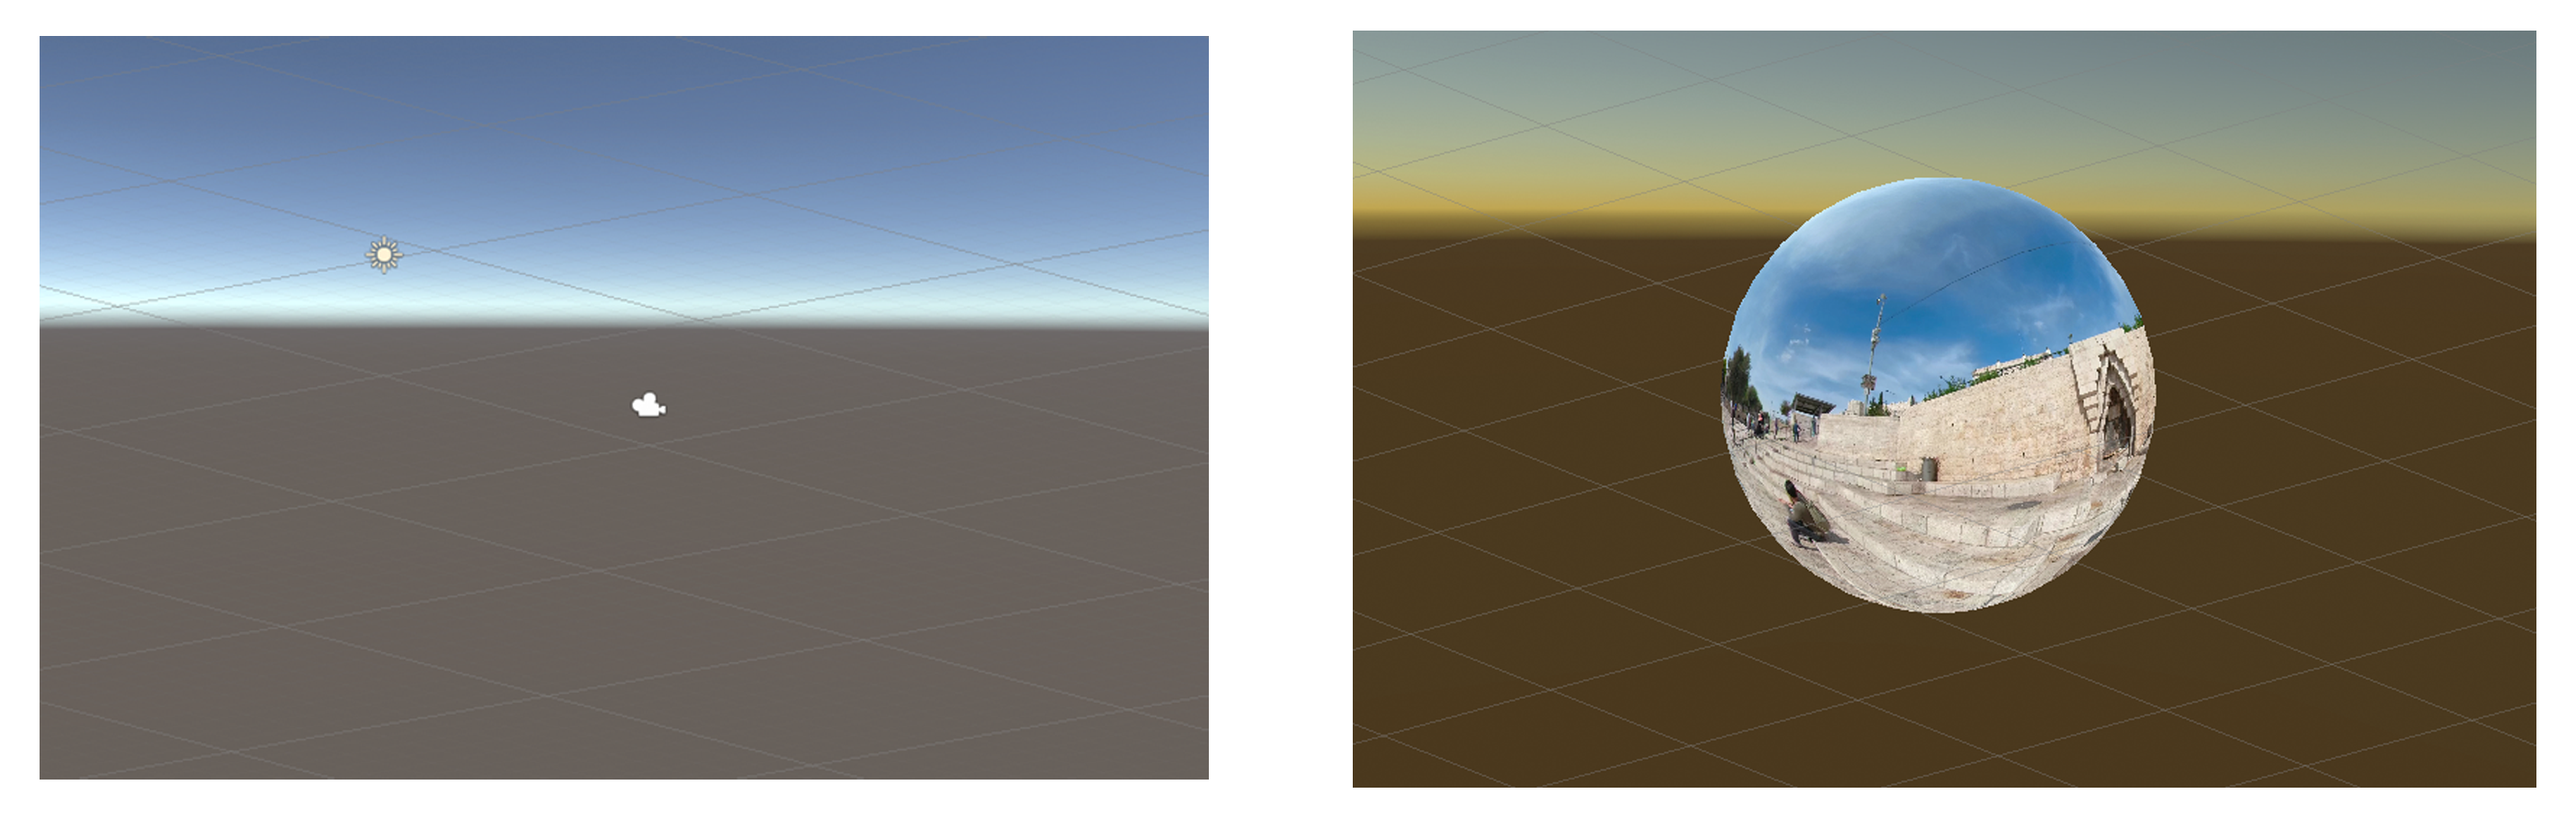
\includegraphics[width=0.90\textwidth]{images/sphere.png}
    \caption{Virtual Reality Sphere in Unity }
    \label{fig:sphere}
\end{figure}


Next, I wanted to design a scene and code it absolutely where I could later use it as a template for other scenes. Before that, I rendered the 360 videos, it took a lot of computer power because it stitched and rendered two videos from the two lenses in the camera. I rendered the videos at night and worked on the application design during the day.

I took the first video to Unity, and it was jamming all the time as I tried it. The image was frozen, then I heard no sound. On a standalone VR video player, I tried to play the video. This performed well, and with sound. I took a step backwards and tested the configuration that I used for rendering. The video was made in a 5.2k quality with spatial sound of 8 audio channels. Unity can not handle 5.2k video seamlessly and without a third-party plug-in, it can not process spatial audio with 8 audio channels. Once I made the rendering configuration changes, I researched the video settings in Unity in the unity community forum and found that the videos had to be trans-coded in Unity, so I trans-coded the videos with VP8 codec. The videos worked smoothly after that. 

Now I have a Virtual Reality environment, I am inside a 360$^{\circ}$ video and I look around me as I am being there. The spatial sound problem, was solved automatically by Unity, the audio of the video was analyzed and it was given the spatial sound functionality, because of spatial sound recording feature in the GoPro Fusion. That means the audio will move where is the user looking at, some people call it \say{3D Sound}.   

Users need to move around different locations and cities, therefore they need a selection tool or a controller. Due to the findings in the first pre-study during \acrfull{yallah!} hackathon, the application needs to be on a smartphone for an easier accessibility and functionality for users. Therefore, it wouldn't be reliable to program the application for a certain kind of controller. Thus, I decided to have a gaze feature in the application. The gaze feature allows the users to select active items or buttons inside the \acrshort{vr} environment only by looking at the button or active item. 


I used the GoogleVR Unity asset to incorporate the environmental gaze functionality. The gaze feature adds a small blue circle in the middle of the vision of users. While the user looks at a button or an active object, an animated white stripe timeline will appear around the circle. It is an interactive sequence of 3 seconds. Once it is done, like a mouse-click on the button or the active item will be triggered. 

I used a default button from Unity for testing the gaze feature. Therefore I created another scene that contains the same components but with a different video. I added a C\# code to the button to give it the functionality of transferring the user between the scenes. 

I was searching for Palestinian villages maps to reconstruct them, but sadly I couldn't find anything on the internet. I've searched blogs, forums, Facebook groups, but no results have been found. Therefore I made contact with a Palestinian expert in the demolished and depopulated villages. Upon describing the application concept to him, he remembered that there is a man used to live in Al-Ghabisiyya village has a map for the village before 1948. I made a contact with the man via WhatsApp, he was very open and showed interest in the project. 
He told me the map was originally based on an Al-Ghabisiyya Ariel photo taken in 1946 by the British mandate. By the end of the day, he sent me a picture for the map via WhatsApp, as shown in Figure \ref{fig:ghmap} the map had numbers on the buildings. Then he sent me a list that contains the family names next to the house numbers that are shown on the map. 
\begin{figure}[ht]
    \centering
    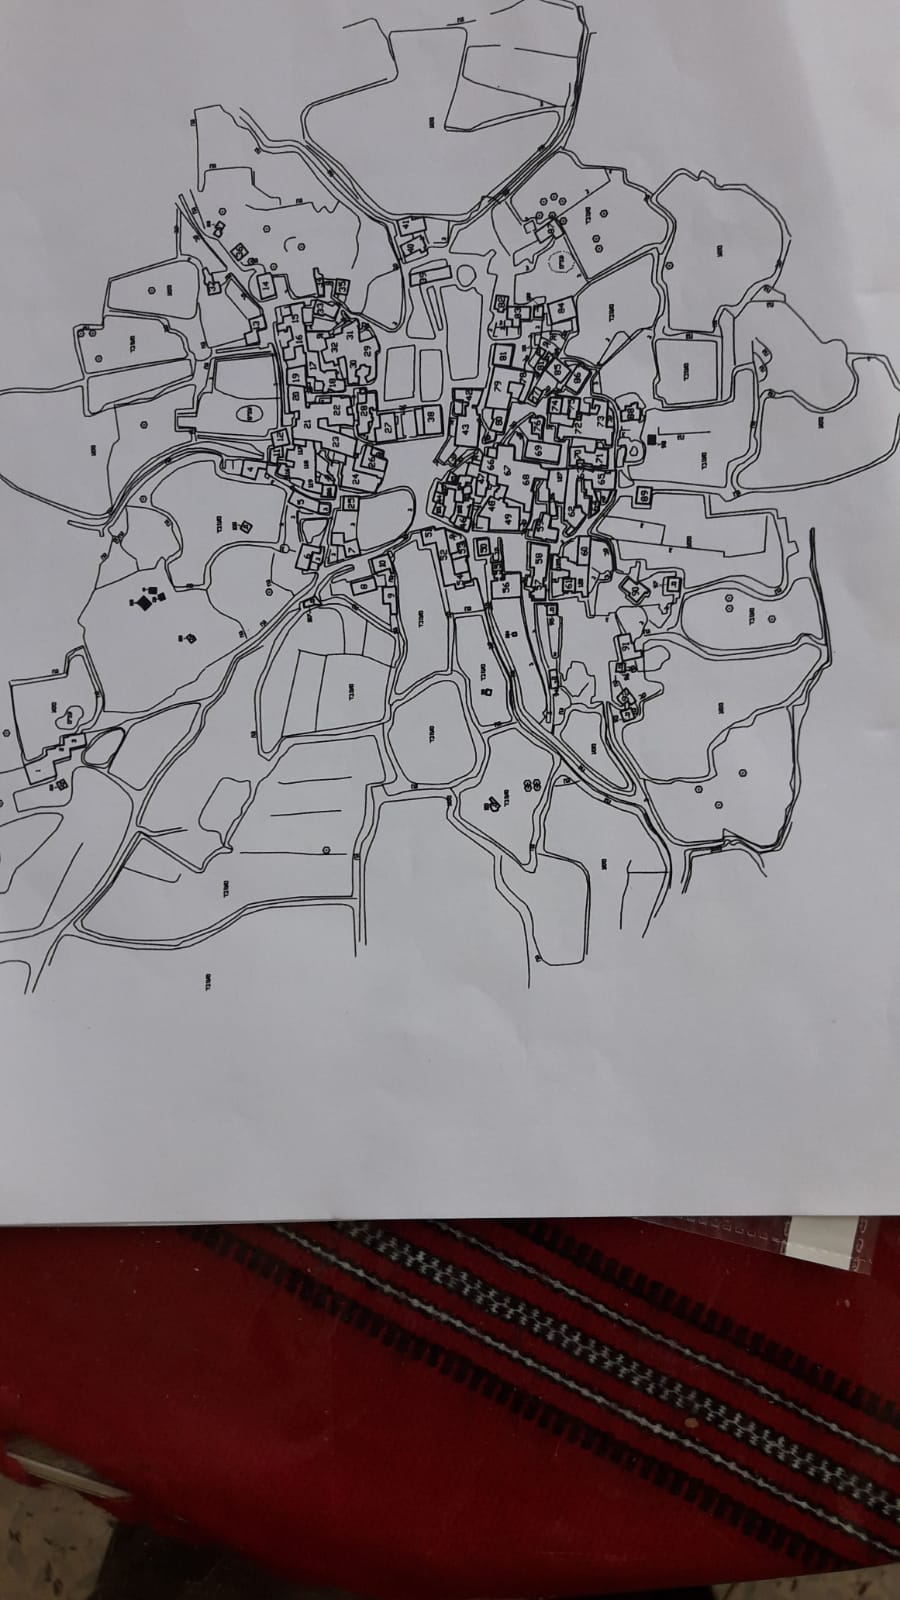
\includegraphics[width=0.50\textwidth, angle=270]{images/ALGHABS_MAP.jpeg}
    \caption{Al-Ghabisiyya Map}
    \label{fig:ghmap}
\end{figure} 
 
He told me during my conversation with the man that the only structure in Al-Ghabisiyya that still stands is the mosque. I scanned through the list to find the mosque number, and it was 38. That's going to be my reference point for the rest of the village for 3D modeling. Palestineremembered.com is a website for offering specific information on each village, it helped me locate Al-Ghabisiyya's place on Google Maps. On Google Maps, I found the mosque, although the whole place now looks like a forest. To align it with the village map, I took a screenshot of the satellite map of the village area.  

The map had no keys for scale or orientation, I didn't know what is the north and what is the west. I thought to try to scale it and use the mosque as a reference, and send it back to the man, to ask him for confirmation. I used Adobe Photoshop to combine the photos to get a better understanding of how did the village look like as shown in Figure \ref{fig:wmap}.     

\begin{figure}[ht]
    \centering
    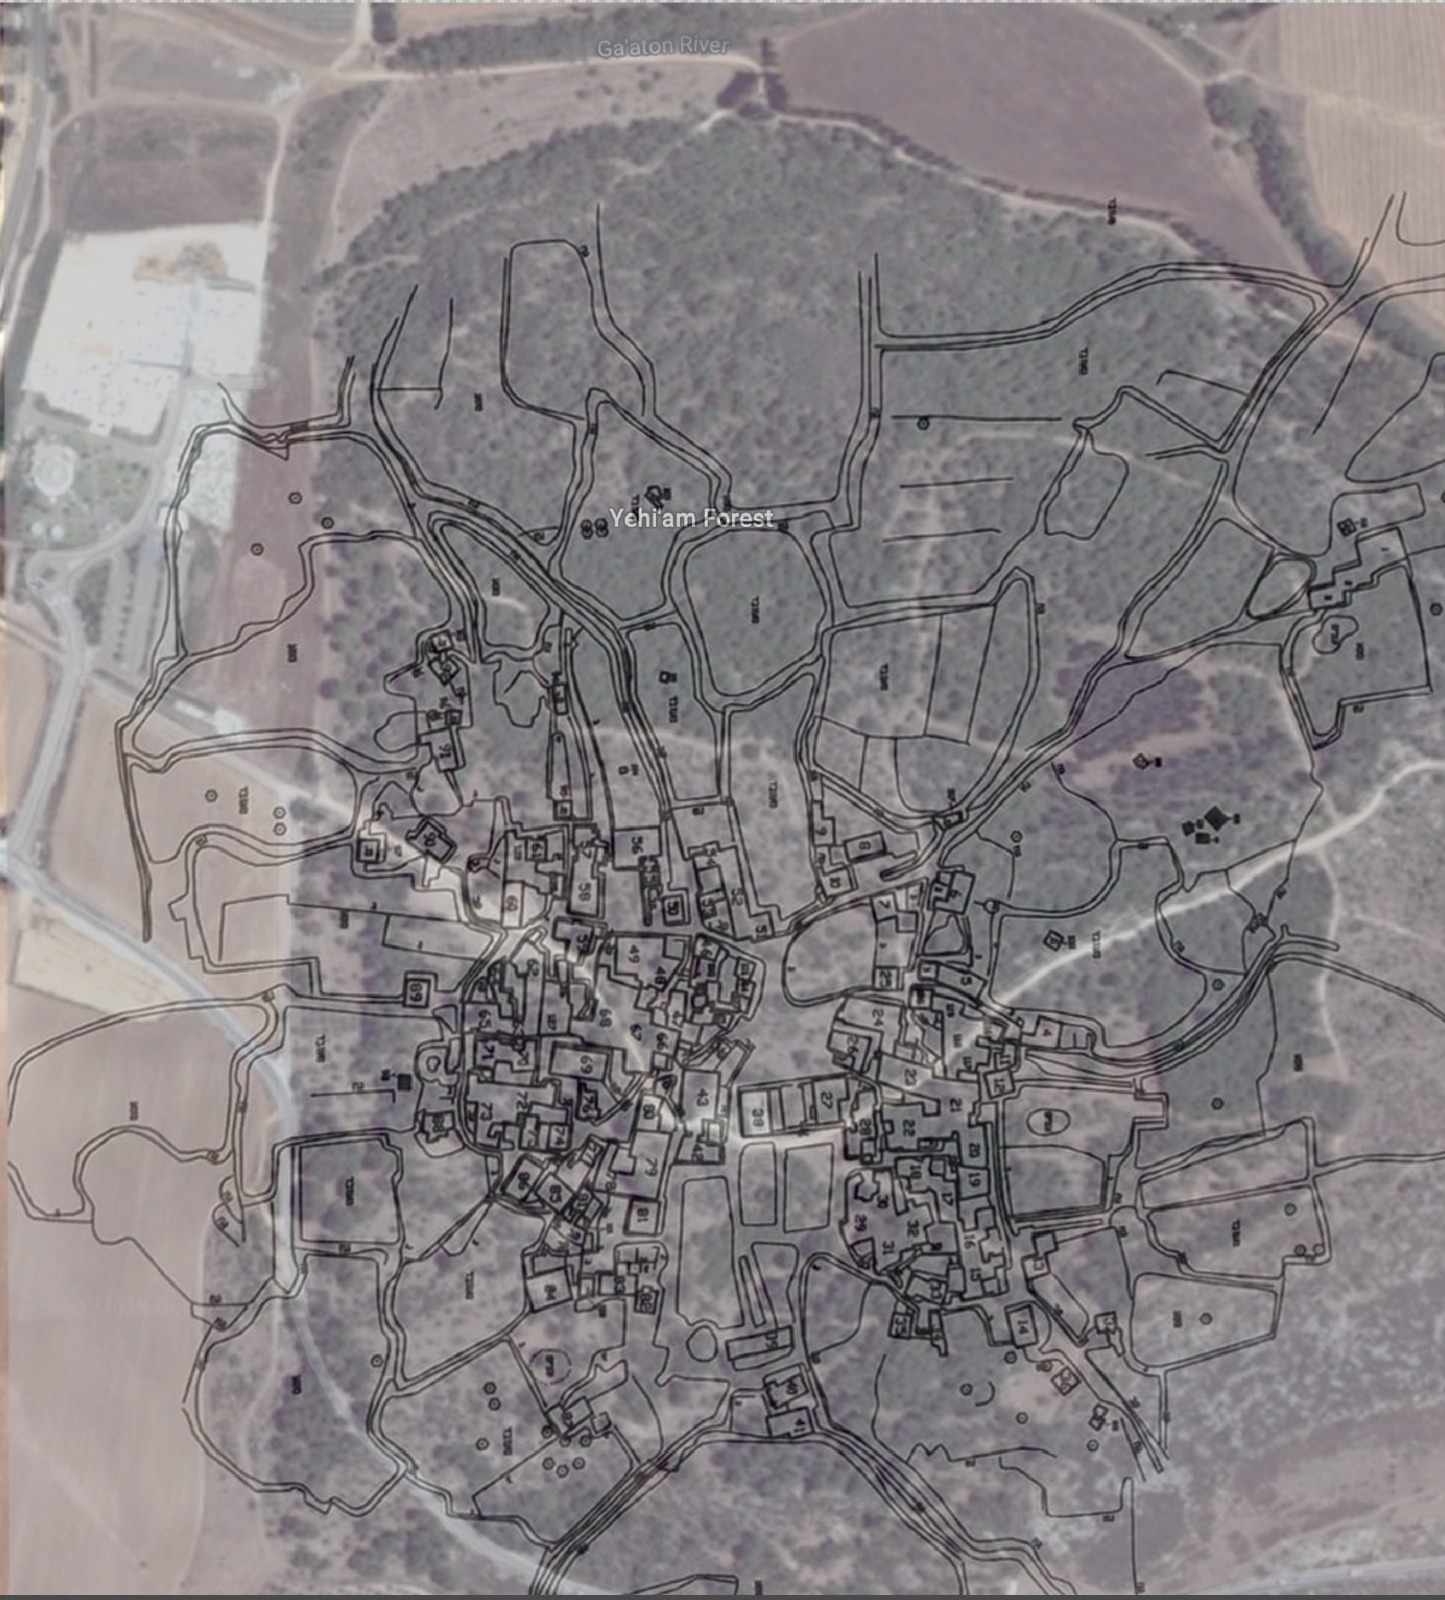
\includegraphics[width=0.60\textwidth]{images/wr_ghb.jpeg}
    \caption{The First try of Mapping Al-Ghabisiyya}
    \label{fig:wmap}
\end{figure} 

Upon getting assurance from the man that the location of the map is right, I started preparing the village ground sketch on Adobe Illustrator as it can export SVG images. Then in Fusion 360, I can import the SVG template and extrude the model so that the buildings have the third dimension. While I was drawing the map on Adobe Illustrator, I discovered that the Mosque's yard was on the map, so I pointed out there was a major error in the mapping I sent to the man. 
The mosque yard is in front of the entrance to the mosque to accommodate as many people during prayers as possible. The entry should be in the direction of Mecca, and the mapping in Figure \ref{fig:wmap} it is in the direction to the west. Therefore, I took a straight line from the mosque to Mecca in Google maps as shown in Figure \ref{fig:stline}, to validate my vision about the map.


\begin{figure}[ht]
    \centering
    \includegraphics[width=1\textwidth]{images/stline.png}
    \caption{Al-Ghabisiyya Mosque Direction to Mecca}
    \label{fig:stline}
\end{figure} 

The mosque position is aligned exactly with the straight line that I drew. This was a validation of the map orientation and scale. I continued to scale down the map and rotate it in the correct position afterward. when I came to the correct orientation and size of the map, It fit perfectly with the geography of the area as shown in Figure \ref{fig:scale} after all those years.


\begin{figure}[ht]
    \centering
    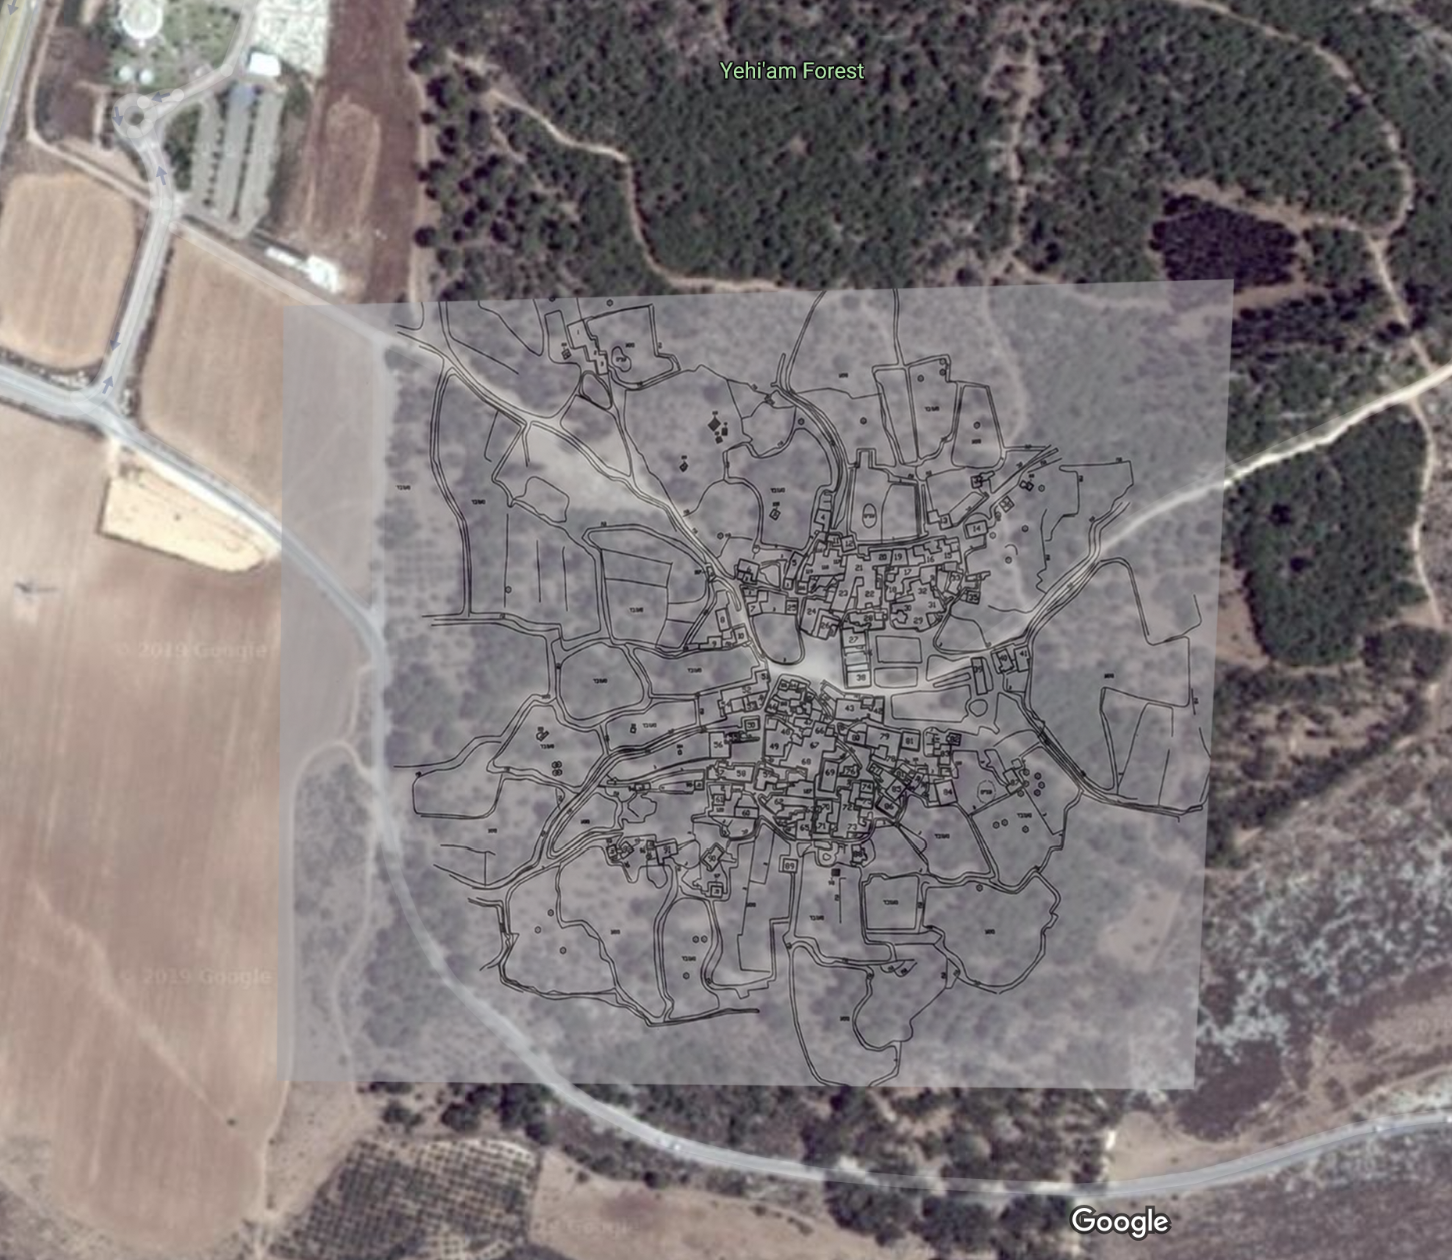
\includegraphics[width=0.70\textwidth]{images/scale.png}
    \caption{Al-Ghabisiyya Mapping Correction}
    \label{fig:scale}
\end{figure} 
 
I started with the village's 3D modeling after refining the map orientation, mapping every house as close as possible to the map I received. Having a high-quality map when working on a significant detail would be better. Unfortunately, it was a picture of low quality, but I tried to get as close as possible to most of the buildings as they appeared. Nevertheless, I couldn't get any more details about the specifications of the buildings, such as doors or windows. I need not only model the village in 3D form, but I need to determine the landscape and the location of the village accurately as well. I used 3D-map-generator.com for getting a depth map for the area as a PNG image. In Unity I used the terrain asset and provide it with the depth map image, for generating the 3D model of the terrain for the area around Al-Ghabisiyya village check Figure \ref{fig:terr}.

\begin{figure}[ht]
    \centering
    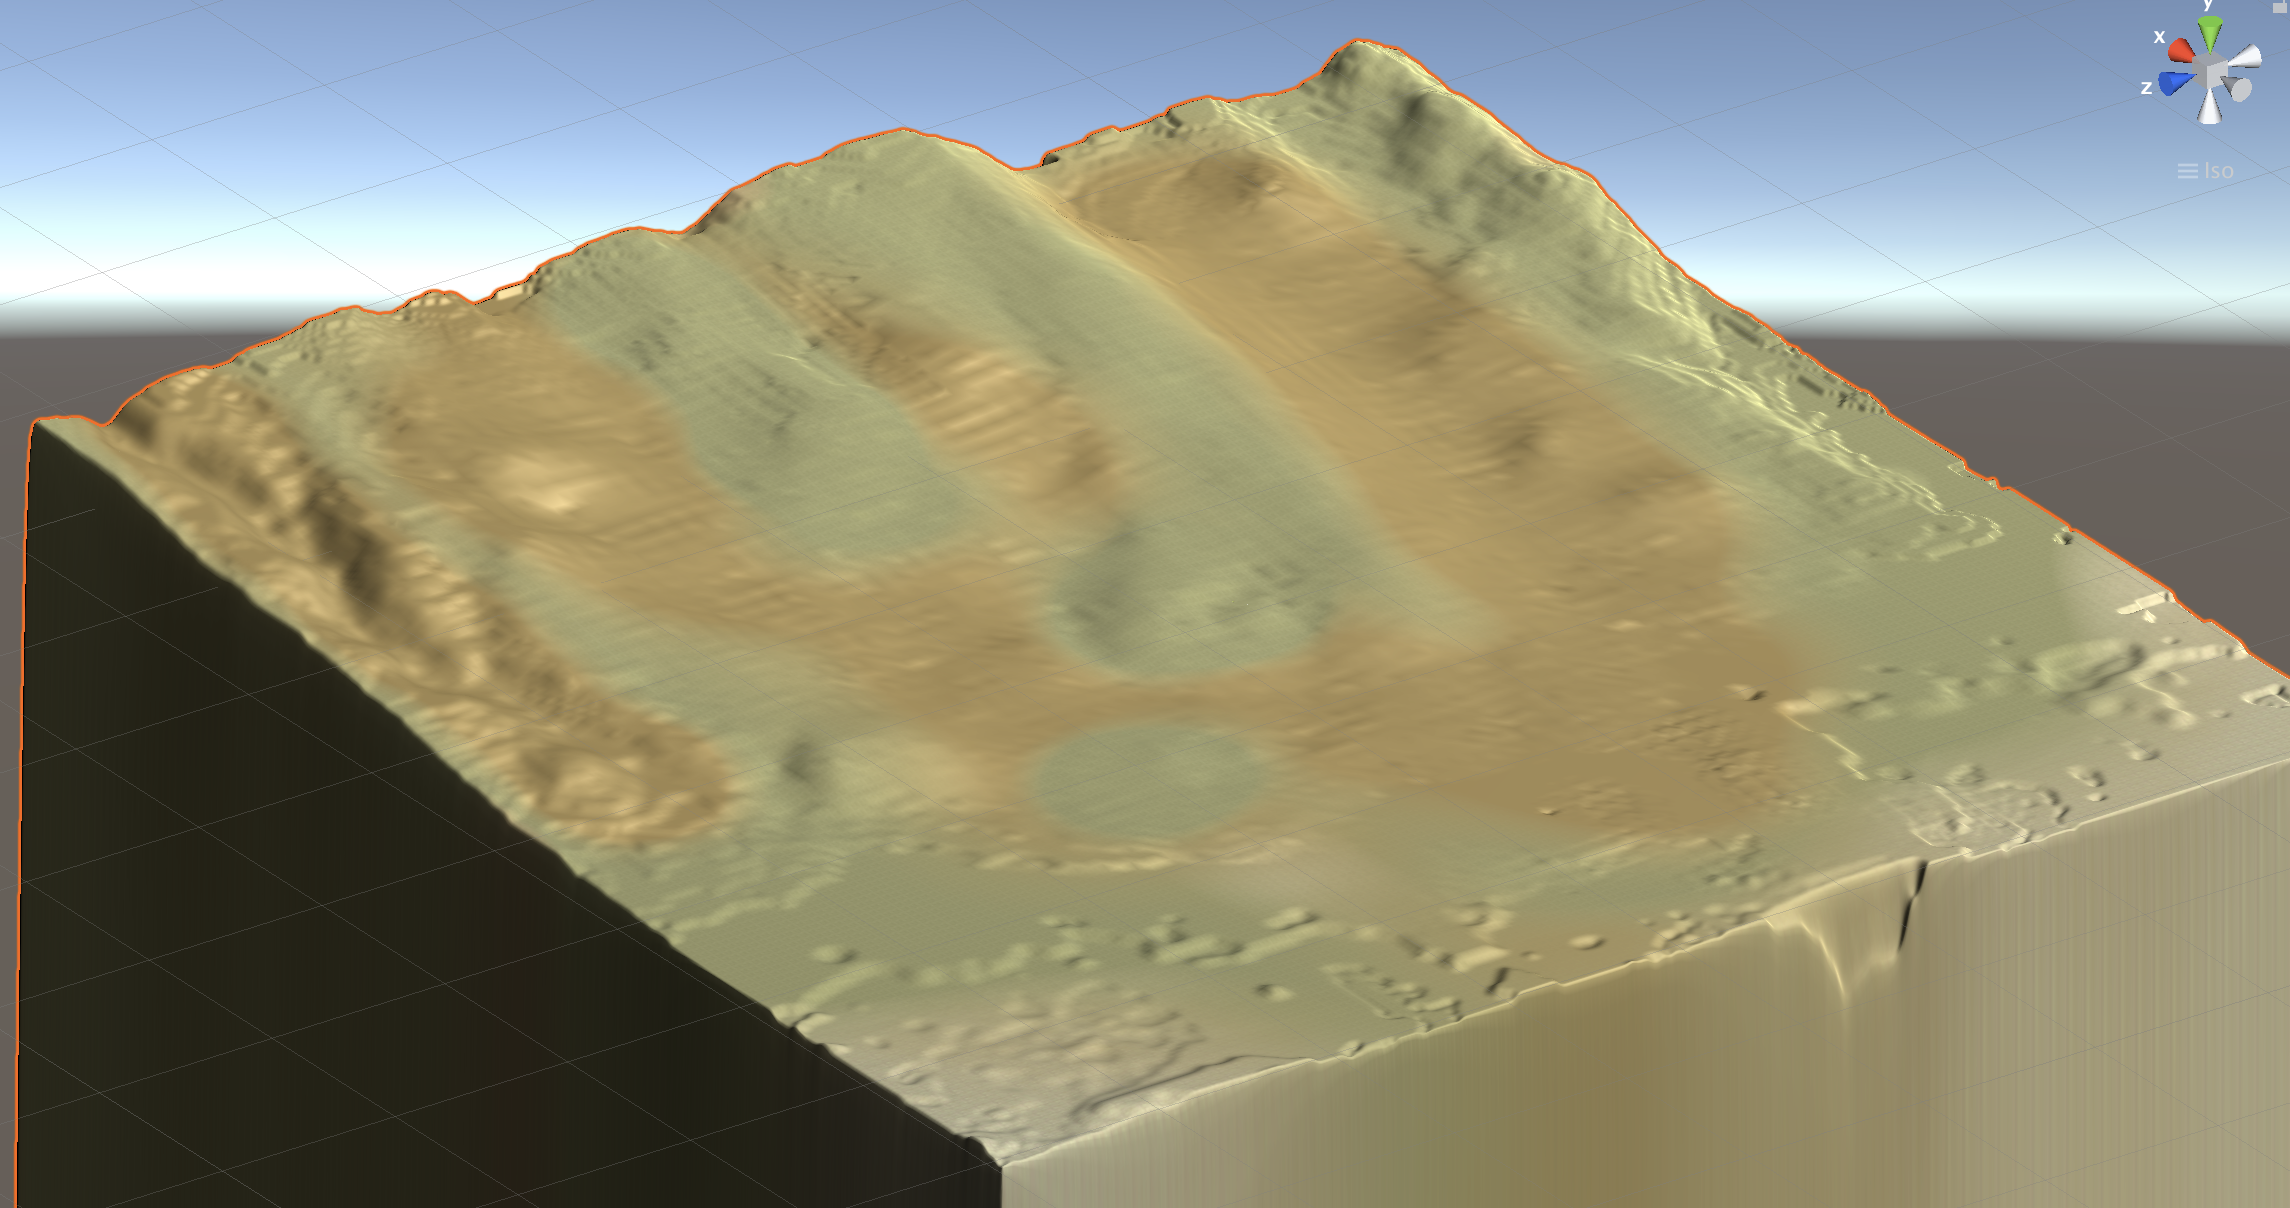
\includegraphics[width=0.70\textwidth]{images/terr.png}
    \caption{Terrain}
    \label{fig:terr}
\end{figure} 


Now I have the terrain of the whole surrounding and I have the village modeled. Placing the village on the terrain with the right scaling needs to be precise. There is no easy way to do that except using the previous way that I did it with the map and the satellite image, by applying the layers over each other in Photoshop. I took an upper screenshot of the terrain and I added it to Photoshop as a third layer on the previous work. I combined between a satellite image, a three dimensional computer generated terrain, and a map for Al-Ghabisiyya. I placed Al-Ghabisiyya model on the right location. I had to take screenshot of the terrain every time I move Al-Ghabisiyya model on the Terrain and compare the location on Photoshop I repeated the process multiple times until I achieved the correct result. The only building that I modeled it with details was the mosque, since it is the only thing that remained in Al-Ghabisiyya, then it was clear for me, the rest of the buildings were modeled as blocks. However I added an old stone texture to the buildings as how I saw the photos of Al-Ghabisiyya mosque photos. 

\begin{figure}[ht]
    \centering
    \includegraphics[width=1\textwidth]{images/Ghab_mos.png}
    \caption{3D model of Al-Ghabisiyya and the Mosque}
    \label{fig:3d}
\end{figure} 

\subsection{User Interface}

\say{In order to allow human-computer interaction it is necessary to use special interfaces designed to input a user's commands into the computer and to provide feedback from the simulation to the user} \citep{burdea2017virtual}.